%-*- coding: UTF-8 -*-
% notes.tex
%
\documentclass[UTF8]{article}
\usepackage{geometry}
\geometry{a4paper, centering, scale=0.8}
\usepackage{minted}
\usepackage{hyperref}
\usepackage{indentfirst}    % to indent the first paragraph of a section
\usepackage{graphicx}       % to insert figures
\usepackage{amsmath}        % to type some math equations
\usepackage{amssymb}        % to use some special math font
\usepackage{IEEEtrantools}  % to use IEEEeqnarray
\usepackage{algorithm2e}    % to use algorithm environment
\usepackage{multicol}       % to display some content in multi-columns
\setlength{\columnseprule}{0.4pt}   % set the rule's width of multicols
\setlength{\columnsep}{5em}         % set the sep of multicols

% Math notation
% refered to https://github.com/exacity/deeplearningbook-chinese/blob/master/math_symbol.tex
\newcommand{\Scalar}[1]{\mathit{#1}}                % Scalar, the default math font
\newcommand{\Vector}[1]{\boldsymbol{\mathit{#1}}}   % Vector
\newcommand{\Matrix}[1]{\boldsymbol{\mathit{#1}}}   % Matrix
\newcommand{\Tensor}[1]{\textsf{\textbf{#1}}}       % Tensor
\newcommand{\Set}[1]{\mathbb{#1}}                   % Set
\newcommand{\Cal}[1]{\mathcal{#1}}                  % Math Cal

% Draw the lines in a matrix, which is composed by a series of vectors
\newcommand{\vRule}{\rule{0.3pt}{10mm}}             % vertical rule
\newcommand{\hRule}{\,\rule[1mm]{10mm}{0.3pt}\,}    % horizontal rule

\title{Deep Learning Specialization \\
        Improving Deep Neural Networks: Hyperparameter tuning, Regularization and Optimization \\
        Learning Notes}
\author{Du Ang \\ \texttt{du2ang233@gmail.com} }
\date{\today}

\begin{document}
\maketitle

\tableofcontents
\newpage

\section{Practical aspects of Deep Learning}
\subsection{Setting up your Machine Learning Application}
\subsubsection{Train/Dev/Test sets}
When training a neural network, you have to make a lot of decisions, such as choosing the number of
layers of the neural network, choosing the number of hidden units of each hidden layer, choosing
the learning rates and activations.

Applied machine learning is a highly iterative process. At first, you have some ideas and make some
decisions. Then you implement the ideas with code in programming. You run some experiments and you
get back a result that tells you how well this particular network, or this particular configuration
works. And based on the outcome, you might refine your ideas and change your choices and maybe keep
iterating in order to try to find a better and beter neural network.

Intuitions from one domain or from one application area often do not transfer to other application
areas. And the best choices may depend on the amount of data you have, the number of input features
you have through your computer configuration and whether you're training on GPUs or CPUs. Even very
experienced deep learning people find it almost impossible to correctly guess the best choice of
hyperparameters the very first time. And so today, applied deep learning is a very iterative
process where you just have to go around this cycle many times to hopefully find a good choice of
network for your application. So one of the things that determine how quickly you can make progress
is how efficiently you can go around this cycle.

Setting up your data sets well in terms of your train, development and test sets can make you much
more efficient at that. The dataset can be separated into three parts: training set, dev set
(development set, hold-out cross validation) and test set.

In the previous era of machine learning, it was common practice to take all your data and split it
accordin to 70/30 percent in terms of a people often talk about the 70/30 train test splits, if you
don't have an explicit dev set. Or maybe a 60/20/20 percent split in terms of 60\% train, 20\% dev
and 20\% test. And several years ago, this was the widely considered as the best practice in
machine learning, if you have 100, 1000 or 10,000 examples.

But in modern big data era, where you might have a million examples in total, then the trend is
that your dev and test sets have been becoming a much smaller percentage of the total. Because
remember, the goal of the dev set is that you're going to test different algorithms on it and see
which algorithm choices works better. So the dev set just needs to to be big enough for you to
evaluate, for example, two different algorithm choices or ten different algorithm choices and
quickly decide which one is doing better. And you might not need a whole 20\% of your data for that.
Similarly, the main goal of your test set is, given your final classifier, to give you a pretty
confident estimate of how well it's doing.

\begin{description}
    \item[Previous era (small exampels): ] training set/dev set/test set : 60/20/20
    \item[Big data era: ] training set/dev set/test set : 98/1/1
\end{description}

One other trend we're seeing in the era of modern deep learning is that more and more people train
on mismatched train and test distributions. Let's say you're building an app that lets users upload
a lot of pictures and your goal is to find pictures of cats in order to show your users. Maybe all
your training set comes from cat pictures downloaded off the Internet, but your dev and test sets
might comprise cat pictures from user using our app. It turns out that a lot of webpages have very
high resolution, very professional, very nicely framed pictures of cats. But maybe your users are
uploading blurrier, lower resolution images just taken with a cell phone camera in a more casual
condition. And so the two distributions of data may be different. The rule of thumb to follow in
this case is to make sure that the dev and test sets come from the same distribution.

Finally, it might be okay to not have a test set. If you have only a dev set but not a test set,
what you do is you train on the training set and then try different model architectures. Evaluate
them on the dev set, and then use that to iterate and try to get to a good model. Because you've
fit your data to the dev set, this no longer gives you an unbiased estimate of performance.

In machine learning world, when you have just a train and a dev set but no separate test set, most
people will call this a training set and they will call the dev set the test set. But what they
actually end up doing is using the test as a hold-out cross validation set. Which maybe isn't
complete a great use of terminology, because they're overfitting to the test set.

Having set up a train dev and test set will allow you to integrate more quickly. It will also allow
you to more efficently measure the bias and variance of your algorithm, so you can more efficiently
select ways to improve your algorithm.

\subsubsection{Bias/Variance}
\begin{figure}[htb]
    \centering
    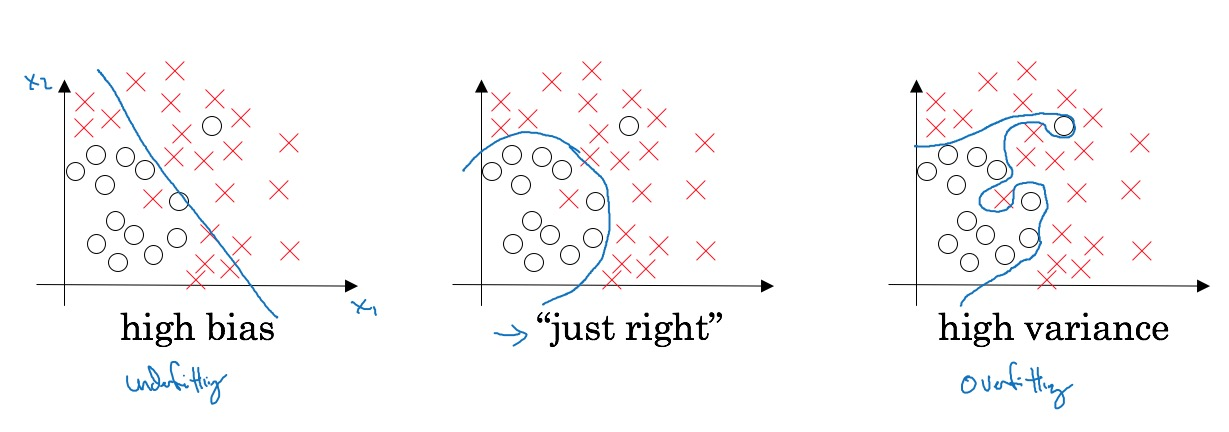
\includegraphics[width=40em]{figures/bias-and-variance-1}
    \caption{Decision boundaries of different classifier on 2D examples}
\end{figure}

\begin{figure}[htb]
    \centering
    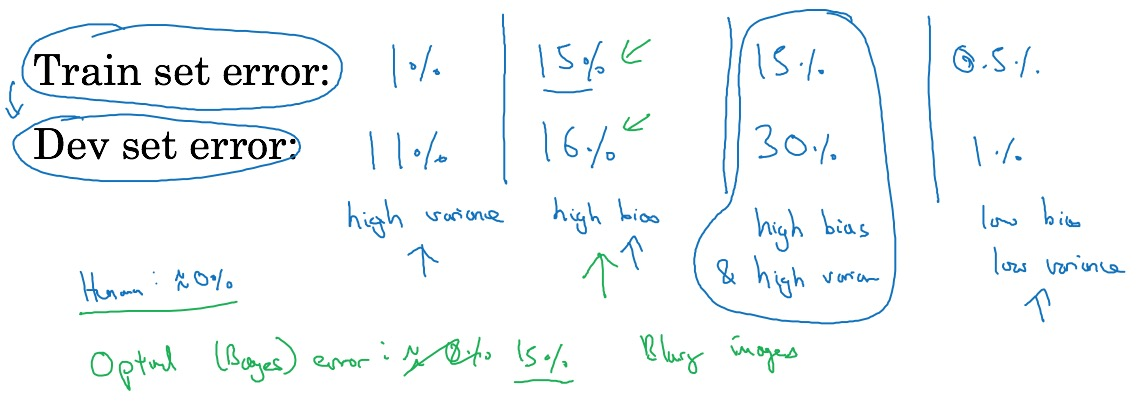
\includegraphics[width=40em]{figures/bias-and-variance-2}
    \caption{Bias or Variance showed by training set error and dev set error. It is related to the
    optimal error (base error), which is determined by the common practices and our expectation.}
\end{figure}

\begin{figure}[htb]
    \centering
    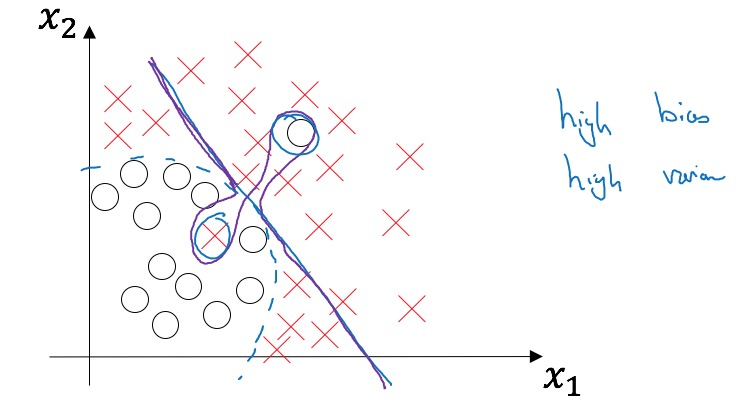
\includegraphics[width=30em]{figures/bias-and-variance-3}
    \caption{The purple decision boundary shows a high bias and high variance case}
\end{figure}

\subsubsection{Basic Recipe for Machine Learning}
\begin{figure}[htb]
    \centering
    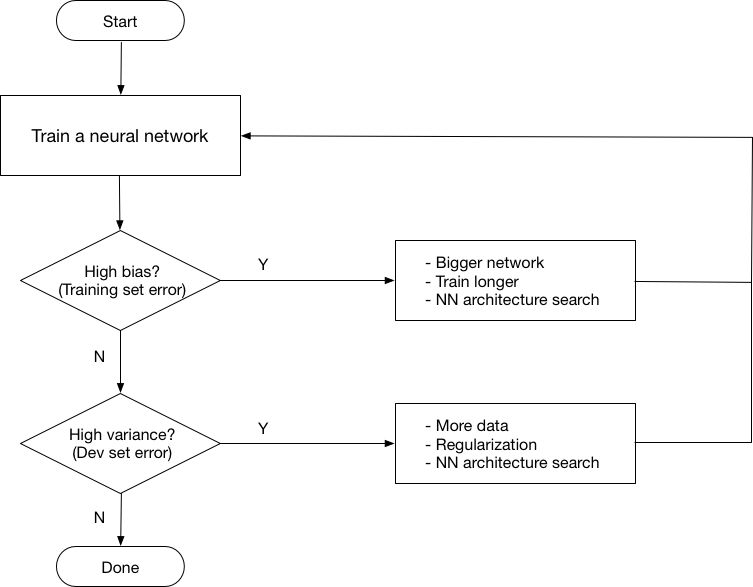
\includegraphics[width=30em]{figures/machine-learning-recipe}
    \caption{Basic recipe for Machine Learning}
    \label{fig:machine-learning-recipe}
\end{figure}

Whereas getting a bigger network almost always helps, and training longer doesn't always help, but
it certainly never hurts. Usually if you have a big enough network, you should usually fit the
training data well so long as it's problem that is possible for someone to do.

If you have high variance problem, the best way to solve high variance problem is to get more data.
But sometimes you can't get more data, or you could try regularization to reduce overfitting. But
if you can find a more appropriate neural network architecture, sometimes that can reduce your
variance problem as well, as well as reduce your bias problem.

Like Figure~\ref{fig:machine-learning-recipe} shows, there are a couple of points to notice. First
is that, depending on whether you have high bias or high variance, the set of things hou should try
could be quite different. So usually use the training dev set to try to diagnose if you have a bias
or variance problem, and then use that to select the appropriate subset of things to try. So for
example, if you actually have a high bias problem, getting more training data is actually not going
to help. Or at least it's not the most efficient thing to do.

\paragraph{Bias variance trade-off} In the earlier era of machine learning, there used to be a lot
of discussion on what is called the bias variance trade-off. And the reason for that was that, for
a lot of the things you could try, you could increase bias and reduce variance, or reduce bias and
increase variance. Back in the pre-deep learning era, we didn't have many tools, we didn't have
as many that just reduce bias or that just reduce variance without hurting the other one. But in
the modern deep learning, big data era, so long as you can keep training a bigger network, and so
long as you can keep getting more data, which isn't always just reduces your bias without
necessarily hurting your variance, so long as you regularize appropriately. And getting more data
always reduces your variance and doesn't hurt your bias much. So what's really happened is that,
with these two steps, the ability to train, pick a network, or get more data, we now have tools to
drive down variance, without really hurting the other thing that much.

\subsection{Regularizing your neural network}
\subsubsection{Regularization}
If you suspect your neural network is overfitting your data, that is you have a high variance
problem, one of the first thing you should try is probably regularization. The other way to address
high variance is to get more training data, which is also quite reliable, but you can't always get
more training data, or it could be more expensive to get more data. But adding regularization
will often help to prevent overfitting, or to reduce the errors in your network.

\paragraph{Logistic regression}
$$ \underset{\Vector{w}, b}{\text{min}} J(\Vector{w}, b) \qquad
\Vector{w} \in \Set{R}^{n_x}, b \in \Set{R} $$
$$ J(\Vector{w}, b) = \frac{1}{m} \sum_{i=1}^m \Cal{L}(\hat{y}^{(i)}, y^{(i)})
+ \frac{\lambda}{2m} ||\Vector{w}||_2^2 $$

\begin{description}
    \item[$L_2$ Norm (squared)]
    $\displaystyle ||\Vector{w}||_2^2 = \sum_{j=1}^{n_x} \Vector{w}_j^2 = \Vector{w}^T \Vector{w} $
    \item[$L_1$ Norm]
    $\displaystyle ||\Vector{w}||_1 = \sum_{j=1}^{n_x}|\Vector{w}_j| $ \qquad
    (Using $L_1$ Norm will make $\Vector{w}$ sparse)
\end{description}

The $\lambda$ means ``regularization parameter'', it helps prevent overfitting. In Python,
\mintinline{python}{lambda} is a reserved keyword, so we use \texttt{lambd}, without \texttt{a}, to
represent the lambda regulzarization parameter.

\paragraph{Neural network}
$$ J(\Matrix{W^{[1]}}, \Vector{b^{[1]}}, \ldots, \Matrix{W}^{[L]}, \Vector{b}^{[L]})
= \frac{1}{m} \sum_{i=1}^{m} \Cal{L}(\hat{\Vector{y}}^{(i)}, \Vector{y}^{(i)})
+ \frac{\lambda}{2m} \sum_{l=1}^L ||\Matrix{W}^{[l]}||_F^2 \qquad
\Matrix{W} \in \Set{R}^{(n^{[l]}, n^{[l-1]})}$$

\begin{description}
    \item[Frobenius Norm (squared)]
    $ \displaystyle ||\Matrix{W}^{[l]}||_F^2 = \sum_{i=1}^{n^{[l-1]}} \sum_{j=1}^{n^{[l]}}
    (\Matrix{W}_{ij})^2 $ \\ (the sum of squares of elements of a matrix, just like $L_2$ norm)
\end{description}

In backpropagation,
$$ \text{d}\Matrix{W}^{[l]} = \frac{1}{m} \text{d}\Matrix{Z}^{[l]} {\Matrix{A}^{[l-1]}}^T
+ \frac{\lambda}{m} \Matrix{W}^{[l]} $$
$$ \Matrix{W}^{[l]} := \Matrix{W}^{[l]} - \alpha \text{d}\Matrix{W}^{[l]} $$

$L_2$ norm sometimes is called ``weight decay'', that's because
\begin{IEEEeqnarray*}{rCl}
\Matrix{W}^{[l]} := \Matrix{W}^{[l]} - \alpha \text{d}\Matrix{W}^{[l]}
= \Matrix{W}^{[l]} - \alpha (\frac{1}{m} \text{d}\Matrix{Z}^{[l]} {\Matrix{A}^{[l-1]}}^T
+ \frac{\lambda}{m} \Matrix{W}^{[l]})
= (1 - \frac{\alpha \lambda}{m}) \Matrix{W}^{[l]}
- \frac{\alpha}{m} \text{d}\Matrix{Z}^{[l]}{\Matrix{A}^{[l-1]}}^T
\end{IEEEeqnarray*}

\subsubsection{Why regularization reduces overfitting?}
\paragraph{Intuition 1}
$$ J(\Matrix{W^{[1]}}, \Vector{b^{[1]}}, \ldots, \Matrix{W}^{[L]}, \Vector{b}^{[L]})
= \frac{1}{m} \sum_{i=1}^{m} \Cal{L}(\hat{\Vector{y}}^{(i)}, \Vector{y}^{(i)})
+ \frac{\lambda}{2m} \sum_{l=1}^L ||\Matrix{W}^{[l]}||_F^2 $$

What we did for regularization was adding extra term $\lambda$ to penalize the weight matricies
$\Matrix{W}^{[l]}$ from being too large. So why is it that shrinking the $L_2$ norm or the
Frobenius norm might cause less overfitting? One piece of intuition is that if you crank
regularization lambda to be really, really big, they'll be really incentivized to set the weight
matricies $\Matrix{W}^{[l]}$ to be reasonably close to zero. So one piece of intuition is maybe it
set the weight to be so close to zero for a lot of hidden units that's basically zeroing out a lot
of the impact of these hidden units. And if that's the case, then this much simplified neural
network becomes a much smaller neural network. In fact, it is almost like logistic regression
units, but stacked most probably as deep. And so that will take you from this overfitting case much
closer to the left to other high bias case, just like Figure~\ref{fig:regularization-intuition-1}.
But hopefully there'll be an intermediate value of lambda that results in a result closer to this
just right case in the middle.

\begin{figure}[htb]
    \centering
    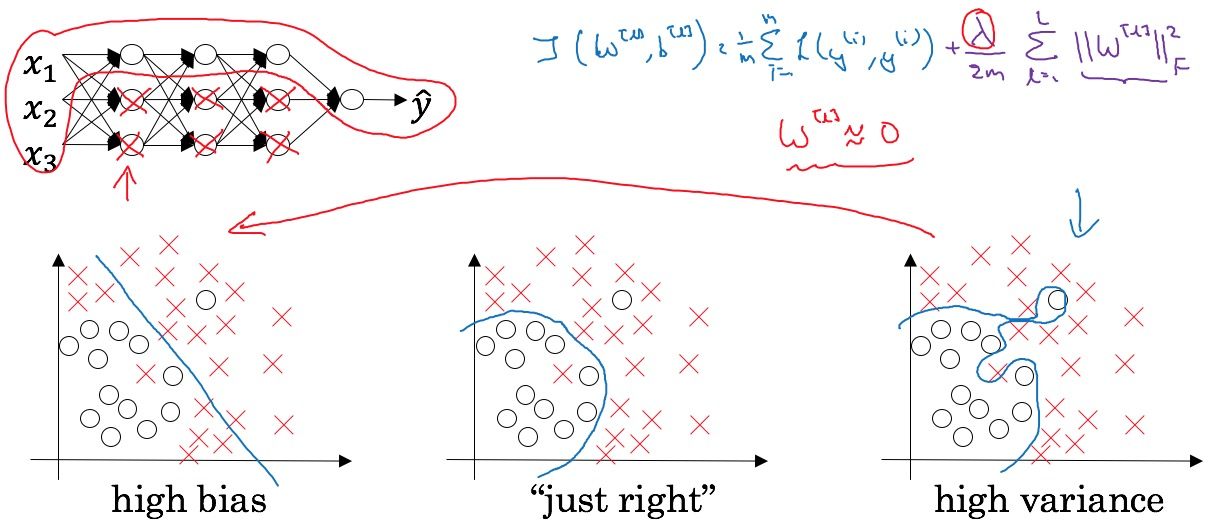
\includegraphics[width=40em]{figures/regularization-intuition-1}
    \caption{A intuition of regularization: big $\lambda$ penalizes weights to almost zeros, make
    it a simpler network}
    \label{fig:regularization-intuition-1}
\end{figure}

\paragraph{Intuition 2}
\begin{figure}[htb]
    \centering
    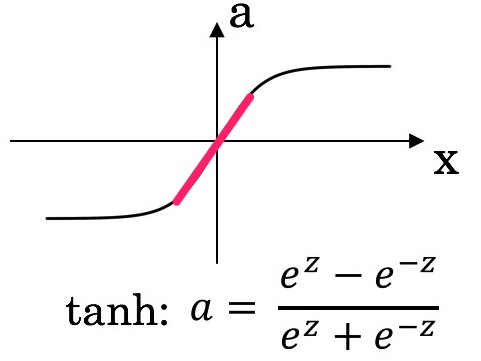
\includegraphics[width=25em]{figures/regularization-intuition-2}
    \caption{A intuition of regularization: big $\lambda$ penalizes weights $\Matrix{W}^{[l]}$
    smaller, then $\Matrix{Z}^{[l]}$ will be smaller and will fall on the linear part of tanh
    activation function}
    \label{fig:regularization-intuition-2}
\end{figure}

In Figure~\ref{fig:regularization-intuition-2}, there is another attempt at additional intuition
for why regularization helps prevent overfitting. And for this, We assume taht we're using the tanh
activation function which looks like this. So if that's the case, if the regularization parameter
$\lambda$ is large, then your parameters $\Matrix{W}^{[l]}$ will be relatively small, then
$\Matrix{Z}^{[l]}$ will be relatively small. And in particular, if $\Matrix{Z}^{[l]}$ ends up
taking relative small values, then $g(\Matrix{Z}^{[l]})$ will be roughly linear. So it's as if
every layer will be roughly linear. We saw in course one that if every layer is linear then your
whole network is just a linear network, as if it is just linear regression. So even a very deep
network, in this case, it will compute something not far from a big linear function which is
therefore pretty simple function rather than a very complex highly non-linear function. And so it
is much less able to overfit.

\subsubsection{Dropout Regularization}
In addition to $L_2$ regularization, another very powerful regularization techniques is called
``dropout''.

Like Figrure~\ref{fig:dropout} shows, with dropout, what we're going to do is go through each of
the layers of the network and set some probability of eliminating a node in neural network. So you
end up with a much smaller, really much diminished network. On different examples, you would toss a
set of coins again and keep a different set of nodes and then dropout or eliminate different set of
nodes. So for each example, you would train it using one of these neural reduced networks.

\begin{figure}[htb]
    \centering
    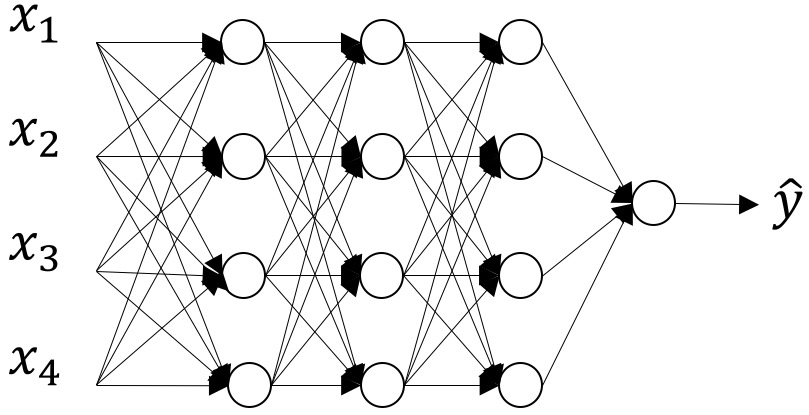
\includegraphics[width=20em]{figures/dropout-orig}
    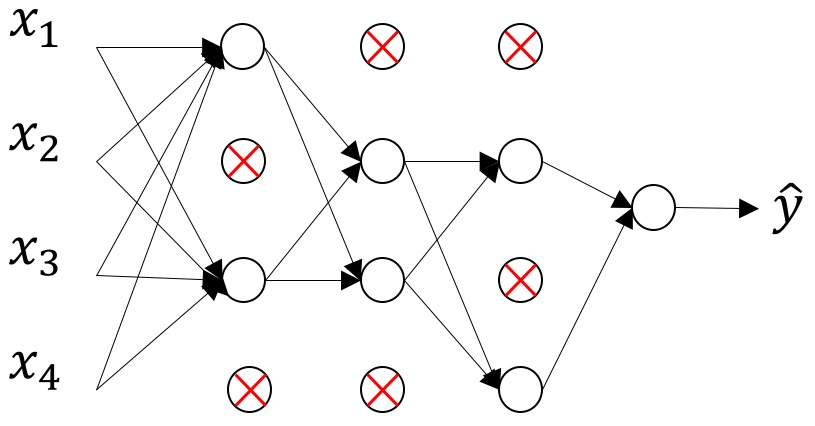
\includegraphics[width=20em]{figures/dropout-zero-out}
    \caption{Dropout}
    \label{fig:dropout}
\end{figure}

\paragraph{Implementing dropout (``Inverted dropout'')}
For the sake of completeness, let's say we want to illustrate this with layer $l=3$. What we are
going to do is set a vector \texttt{d3}, which is going to be the dropout vector for the
layer 3.
\begin{minted}{numpy}
    keep_prob = 0.8  # the probability of keeping each unit

    d3 = np.randm.rand(a3.shape[0], a3.shape[1]) < keep_prob
    a3 = np.multiply(a3, d3)  # a3 * d3, element-wise multiplication
    a3 /= keep_prob  # inverted dropout
\end{minted}

\paragraph{Making predictions at test time}
Don't use dropout at test time. That's because when you are making predictions at the test time,
you don't really want your output to be random. If you are implementing dropout at test time, that
just add noise to your predictions. In theory, one thing you could do is run a prediction process
many times with different hidden units randomly dropped out and have it across them. But that's
computationally inefficient and will give you roughly the same result.

And just to mention, the inverted dropout thing, you remember the step on the previous line when we
divided by the \texttt{keep\_prob}. The effect of that was to ensure that even when you don't
implement dropout at test time to the scaling, the expected value of the activations don't change.
So you don't need to add an extra funny scaling parameter at test time.

\subsubsection{Understanding dropout}
Intuition: Can't rely on any one feature, so have to spread out weights. And by spreading norm of
the weights, this will tend to have an effect of shrinking the squared norm of the weights. And so,
similar to what we saw with $L_2$ regularization, the effect of implementing dropout is that it
shrinks the weights and does similar to $L_2$ regularization that helps prevent overfitting.
But it turns out that dropout can formally be shown to be an adaptive form without a regularization,
while $L_2$ penalty on different weights are different, depending on the size of the activations
being multiplied that way.

It is also feasible to vary \texttt{keep\_prob} by layer. The \texttt{keep\_prob} of $1.0$ means
that you're keeping every unit and so you're really not using dropout for that layer. But for
layers where you're more worried about overfitting, really the layers with a lot of parameters, you
can set the \texttt{keep\_prob} to be smaller to apply a more powerful form of dropout.

And technicall, you can also apply droput to the input layer, where you can have some chance of
just maxing out one or more of the input features. Although in practice, usually don't do that that
often. And so, a \texttt{keep\_prob} of $1.0$ was quite common for the input layer.

One downside of dropout is, this gives you even more hyperparameters to search for using
cross-validation. One other alternative might be to have some layers where you apply dropout and
some layers where don't apply dropout, and then you just have one hyperparameter, which is a
\texttt{keep\_prob} for the layers for which you do apply dropouts.

Many of the first successful implementations of dropout were to computer vision, and it is
frequently used by computer vision. But the really thing to remember is that dropout is a
regularization technique, it helps prevent overfitting, don't use it unless your algorithm is
overfitting.

Another big downside of dropout is that the cost function $J$ is no longer well-defined. On every
iteration, you are randomly killing off a bunch of nodes. And so, if you are double checking the
performance of gradient descent, it will be harder to double check that because the cost function
$J$ is less well-defined or is certainly hard to calculate. So we lose the debugging tool to plot
the graph $J$ of the number of iterations. We can turn off dropout (set \texttt{keep\_prob} equals
$1.0$) at first, and run the code to make sure that it is monotonically decresing $J$. Then turn on
dropout and use other ways, but not plotting the figures, to make sure that our code is working,
the gradient descent is working even with dropout.

\subsubsection{Other regularization methods}
\paragraph{Data augmentation}
Let's say you are fitting a cat classifier. If you are overfitting, getting more data can help, but
getting more training data can be expensive and sometimes you just can't get more data. Then like
Figure~\ref{fig:data-augmentation} shows, we can use data augmentation by using flipping, random
cropping, distortion, etc. to get more training data.

\begin{figure}[htb]
    \centering
    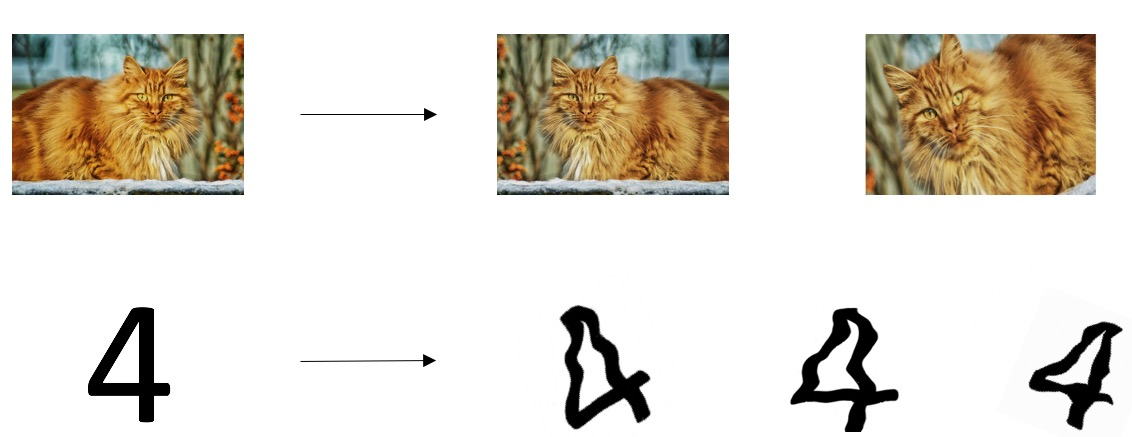
\includegraphics[width=40em]{figures/data-augmentation}
    \caption{Data augmentation}
    \label{fig:data-augmentation}
\end{figure}















\end{document}
